%%%%%%%%%%%%%%%%%%%%%%%%%%%%%%%%%%%%%%%%%
% Short Sectioned Assignment
% LaTeX Template
% Version 1.0 (5/5/12)
%
% This template has been downloaded from:
% http://www.LaTeXTemplates.com
%
% Original author:
% Frits Wenneker (http://www.howtotex.com)
%
% License:
% CC BY-NC-SA 3.0 (http://creativecommons.org/licenses/by-nc-sa/3.0/)
%
%%%%%%%%%%%%%%%%%%%%%%%%%%%%%%%%%%%%%%%%%

%----------------------------------------------------------------------------------------
%	PACKAGES AND OTHER DOCUMENT CONFIGURATIONS
%----------------------------------------------------------------------------------------

\documentclass[letterpaper, fontsize=11pt]{scrartcl} % A4 paper and 11pt font size

\usepackage[T1]{fontenc} % Use 8-bit encoding that has 256 glyphs
\usepackage{fourier} % Use the Adobe Utopia font for the document - comment this line to return to the LaTeX default
\usepackage[english]{babel} % English language/hyphenation
\usepackage{amsmath,amsfonts,amsthm} % Math packages

\usepackage{lipsum} % Used for inserting dummy 'Lorem ipsum' text into the template
\usepackage[margin=1in]{geometry} %set margins -TA
\usepackage{sectsty} % Allows customizing section commands
\allsectionsfont{\centering \normalfont\scshape} % Make all sections centered, the default font and small caps
\usepackage{enumitem}
\usepackage{fancyhdr} % Custom headers and footers
\usepackage{graphicx}
\usepackage{float}

\usepackage{graphicx} % Required to insert images
\usepackage{multicol}
\usepackage{enumitem}
\usepackage{amssymb}
\usepackage{bm}
\usepackage{verbatim}
\usepackage{hyperref}
\usepackage{color}
\usepackage[]{mcode} %MATLAB code

\allowdisplaybreaks


\pagestyle{fancyplain} % Makes all pages in the document conform to the custom headers and footers
\fancyhead{} % No page header - if you want one, create it in the same way as the footers below
\fancyfoot[L]{\textit{CME 102 Spring '15-'16}} % Empty left footer
\fancyfoot[C]{} % Empty center footer
\fancyfoot[R]{Tim Anderson} % Page numbering for right footer
\renewcommand{\headrulewidth}{0pt} % Remove header underlines
\renewcommand{\footrulewidth}{0pt} % Remove footer underlines
\setlength{\headheight}{14pt} % Customize the height of the header

\numberwithin{equation}{section} % Number equations within sections (i.e. 1.1, 1.2, 2.1, 2.2 instead of 1, 2, 3, 4)
\numberwithin{figure}{section} % Number figures within sections (i.e. 1.1, 1.2, 2.1, 2.2 instead of 1, 2, 3, 4)
\numberwithin{table}{section} % Number tables within sections (i.e. 1.1, 1.2, 2.1, 2.2 instead of 1, 2, 3, 4)

\setlength\parindent{0pt} % Removes all indentation from paragraphs - comment this line for an assignment with lots of text
\begin{document}

%----------------------------------------------------------------------------------------
%	TITLE SECTION
%----------------------------------------------------------------------------------------

\newcommand{\horrule}[1]{\rule{\linewidth}{#1}} % Create horizontal rule command with 1 argument of height

%---------------------------------------------------------------------------------------a-
%	PROBLEM 1
%----------------------------------------------------------------------------------------

\section*{Final Review Problems}
\par If not otherwise specified, solve the following problems. If initial conditions are given, solve for all constants of integration. It is okay to leave answers in implicit form or with unsolved integrals. 

\begin{enumerate}

\item \textbf{Direction fields and Equilibrium solutions:} \par Identify the equilibrium solutions and state their type.
\begin{enumerate}

\item For the following figure:
\begin{figure}[h]
\centering 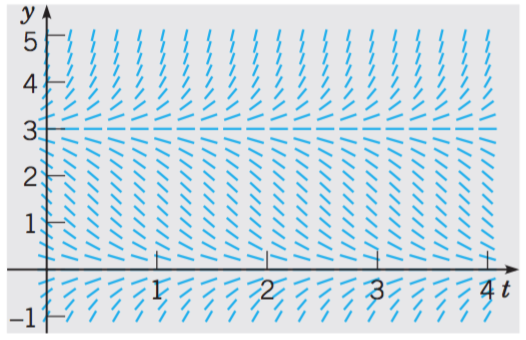
\includegraphics[width = 0.4\columnwidth]{finalReview1.png}
\end{figure}
\par \textbf{Solution:} Unstable equilibrium at $y = 3$ and stable equilibrium at $y = 0$. 
\item  $y' = y(y-2)^2$
\par \textbf{Solution:} There is an unstable equilibrium at $y=0$ and semistable equilibrium at $y = 2$.

\item $y' = y(y - 3)(y-x)$ 
\par \textbf{Solution:} The equation is not autonomous, so there are no equilibrium points. 

\end{enumerate}

\item \textbf{Solution verification:} Verify the solution to the following ODEs. 
\begin{enumerate}

% T&P equation 3.32
\item $x^2y''  + 2xy'  + y = \ln(x) + 3x + 1,\quad y = \ln(x) + x$
\par \textbf{Solution:} 
\begin{gather*}
x^2y''  + 2xy'  + y = \ln(x) + 3x + 1 \\
y = \ln(x) + x \\
y' = \frac{1}{x} + 1\\
y'' = -\frac{1}{x^2} \\
x^2\left(-\frac{1}{x^2}\right)  + 2x\left(\frac{1}{x} + 1\right)  + \ln(x) + x = \ln(x) + 3x + 1 \\
\ln(x) + 3x + 1  = \ln(x) + 3x + 1 \quad\blacksquare
\end{gather*}

% T&P example 3.5
\item $(y'')^3 + (y')^2 - y - 3x^2 - 8 = 0, \quad y = x^2$
\par \textbf{Solution:}
\begin{gather*}
(y'')^3 + (y')^2 - y - 3x^2 - 8 = 0\\
y = x^2\\
y' = 2x\\
y'' = 2\\
(2)^3 + (2x)^2 - x^2 - 3x^2 -8 = 0\\
0 = 0 \quad\blacksquare
\end{gather*}

% T&P example 3.52
\item $y' = (x+y)^2,\quad y = \tan(x) - x$
\par \textbf{Solution}
\begin{gather*}
y' = (x+y)^2 \\
y = \tan(x) - x\\
y' = \sec^2(x) - 1
\sec^2(x) - 1 = (x+\tan(x) -x)^2\\
\sec^2(x)-1 = \tan^2(x) \\
1 - \cos^2(x) = \sin^2(x) \\
1 = 1\quad\blacksquare
\end{gather*}
\end{enumerate}

\item \textbf{Separation of variables:} Solve the following ODEs using separation of variables. 
\begin{enumerate}

\item $y' + y^2 \sin(x) = 0$ 
\par \textbf{Solution:}
\begin{gather*}
y' + y^2 \sin(x) = 0\\
y' = -y^2 \sin(x)\\
\frac{dy}{y^2} = -\sin(x)dx\\
\frac{1}{y} = \cos(x) + C\\
y = \frac{1}{\cos(x) + C}\quad\blacksquare
\end{gather*}

\item $y' =2+2x+2y^2 + 2xy^2, \quad y(0) = 0$
\par \textbf{Solution:}
\begin{align*}
y' &=2+2x+2y^2 + 2xy^2 \\
&= 2(1 + x + y^2 + xy^2)\\
&= 2(1+x)(1+y^2)\\
\frac{dy}{1+y^2} &= 2(1+x)dx\\
\tan^{-1}(y) &= 2x + x^2 + C\\
y &= \tan(2x + x^2 + C)\\
y(0) = 0&=  \tan( C) \implies C = 0\\
y&= \tan(2x + x^2) \quad\blacksquare
\end{align*}

\item $y' =\frac{ty(4-y)}{1+t}$
\par \textbf{Solution:}
\begin{align*}
y' &= \frac{ty(4-y)}{1+t}\\
\frac{dy}{y(4-y)} &= \frac{t}{1+t}dt\\
\intertext{Performing partial fraction decomposition on the left hand side:}
\left( \frac{1}{4y} - \frac{1}{4(y-4)} \right) &= \frac{t}{1+t}dt\\
\intertext{and integrating the right hand side with integration by parts:}
\frac{1}{4}\left( \ln(y) - \ln(y-4)\right) &= t - \ln(t+1) + C\\
\ln\left(\frac{y}{y-4}\right) &= 4t - 4\ln(t+1) + C\quad\blacksquare
\end{align*}

\end{enumerate}

\item \textbf{Existence and uniqueness:} Give the interval for existence and interval for uniqueness of the solution. 
\begin{enumerate}

\item $\sin(2x)dx+\cos(3y)dy=0, \quad y(\pi/2) = \pi/3$
\par \textbf{Solution:} We first need to rearrange the equation to be in the form $y' = f(x,y)$, then we can do our existence and uniqueness tests:
\begin{gather*}
\sin(2x)dx+\cos(3y)dy=0 \\
\cos(3y)dy = -\sin(2x)dx\\
y' = -\frac{\sin(2x)}{\cos(3y)}
\end{gather*}
For existence, $y'$ is discontinuous at $y = \frac{n\pi}{6}$ for $n$ odd. Because our initial condition must lie within our region of existence, the solution thus exists for all $x \in \mathbb{R}$ and for $y \in [\frac{\pi}{6},\frac{\pi}{2}]$. $\quad\blacksquare$
\par For uniqueness, we first need to find $\partial f /\partial y$, then we can find the interval for uniqueness:
\begin{gather*}
y' = -\frac{\sin(2x)}{\cos(3y)}\\
\frac{\partial}{\partial y}y' = -3\sin(2x)\sec(3y)\tan(3y) = -\frac{3\sin(2x)\sin(3y)}{\cos^2(3y)}
\end{gather*}
\par This is discontinuous at the same points as $y'$, so the interval for uniqueness will be the same. 

\item $y^2(1 - x^2)^{1/2}dy = \sin^{-1} (x) dx, \quad y(0) = 1$
\par \textbf{Solution:}
\begin{gather*}
y^2(1 - x^2)^{1/2}dy = \sin^{-1} (x) dx\\
y' = \frac{\sin^{-1}(x)}{y^2(1-x^2)^{1/2}}\\
\frac{\partial}{\partial y} y' = -2\frac{\sin^{-1}(x)}{y^3(1-x^2)^{1/2}}
\end{gather*}
Solution exists for $x \in (-1,1)$ and $y > 0$, and is unique for the same interval. $\quad\blacksquare$

\end{enumerate}

% First order and Bernoulli equation
\item \textbf{Linear first order ODEs:} Solve the following.
\begin{enumerate}

% B&D 2.1 example #3
\item $y' -2y = 4-t$
\par \textbf{Solution:}
\begin{gather*}
y' -2y = 4-t\\
y = e^{-\int (-2)dt}\left[ \int e^{\int(-2)dt}(4-t)dt + C\right] \\
y = e^{2t}\left[ \int e^{-2t}(4-t)dx + C\right] \\
y = e^{2t}\left[ -\frac{7}{4}e^{-2t} + \frac{1}{2}te^{-2t} + C \right] \\
y(t) = -\frac{7}{4} + \frac{t}{2} + Ce^{2t} \quad\blacksquare
\end{gather*}

%B&D 2.1 #18
\item $ty' + 2y = \sin(t),\quad y(\pi/2) = 0, \quad t> 0$
\par \textbf{Solution:} We first need to put the ODE into standard form, then we can easily solve.
\begin{align*}
ty' + 2y &= \sin(t) \\
y' + \frac{2}{t}y &= \frac{\sin(t)}{t}\\
y(t) &= e^{-\int\frac{2}{t}dt} \left[ \int e^{\int \frac{2}{t}dt}\frac{\sin(t)}{t}dt + C\right] \\
&= \frac{1}{t^2} \left[ \int t\sin(t)dt + C\right] \\
&= \frac{1}{t^2} \left[ \sin(t) - t\cos(t) + C\right] \\
&= \frac{\sin(t)}{t^2} - \frac{\cos(t)}{t} + \frac{C}{t^2} \\
y(\pi/2) &= \frac{1}{(\pi/2)^2} + \frac{C}{(\pi/2)^2} = 0 \\
\implies C&= -1\\
y(t) &= \frac{\sin(t)}{t^2} - \frac{\cos(t)}{t} - \frac{1}{t^2} \quad\blacksquare
\end{align*}

\item $ty' + (t+1)y = t,\quad y(\ln(2)) = 1, \quad t> 0$
\par \textbf{Solution:} Putting into standard form then solving...
\begin{align*}
ty' + (t+1)y &= t\\
y' + \frac{t+1}{t}y &= 1\\
y(t) &= e^{-\int\frac{t+1}{t}dt}\left[ \int e^{\int \frac{t+1}{t}dt}(1)dt + C\right] \\
 &= e^{-\int\left(1 + \frac{1}{t}\right)dt}\left[ \int e^{\int \left(1 + \frac{1}{t}\right)dt}dt + C\right] \\
 &= e^{-(\ln(t) +t)}{t}\left[ \int te^{t}dt + C\right] \\
  &= \frac{e^{-t}}{t}\left[ te^t - e^t + C\right] \\
    &= 1 - \frac{1}{t} + \frac{Ce^{-t}}{t} \\
y(\ln(2)) &= 1 - \frac{1}{\ln(2)} + \frac{Ce^{-\ln(2)}}{\ln(2)} =1 \\
\implies C&= 2\\
y(t) &= 1 - \frac{1}{t} + \frac{2e^{-t}}{t} \quad\blacksquare
\end{align*}

\end{enumerate}


% B&P 7.5 example 2 
\item \textbf{Eigenvector solution to ODEs:} Solve the following using an eigenvalue/vector system.

\[
\vec x' = \left[ \begin{array}{cc} 1 & 1 \\ 4 &1 \end{array} \right] \vec x
\]
\par \textbf{Solution:} We know the form of the solution, so all we need to do is find the eigenvalues and eigenvectors and we're done.
\begin{align*}
A - \lambda I &= \left[ \begin{array}{cc} 1 & 1 \\ 4 &1 \end{array} \right] - \lambda \left[ \begin{array}{cc}1 & 0 \\ 0 &1 \end{array} \right] \\
&= \left[ \begin{array}{cc} 1-\lambda & 1 \\ 4 &1-\lambda \end{array} \right] \\
det\left[ \begin{array}{cc} 1-\lambda & 1 \\ 4 &1-\lambda \end{array} \right] &= (1-\lambda)^2 - 4\\
&= \lambda^2 - 2\lambda + 1 - 4\\
&= \lambda^2 -2 \lambda -3\\
&= (\lambda-3)(\lambda +1)\\
\lambda &= -1,\; 3\quad\blacksquare
\end{align*}
For $\lambda_1 = -1$:
\begin{align*}
A - \lambda I &= \left[ \begin{array}{cc} 2 & 1 \\ 4 &2 \end{array} \right]\\
\left[ \begin{array}{cc} 2 & 1 \\ 4 &2 \end{array} \right] \vec v_1&= 0\\
\textbf{Let:} \; \vec v_{1,1} &= 1\\
\intertext{Then from the first line of the matrix equation:}
2v_{1,1} + v_{1,2} &= 0\\
2(1) + v_{1,2} &= 0\\
v_{1,2} &= -2\\
\vec v_1 &= \left[ \begin{array}{c} 1\\ -2 \end{array} \right]
\end{align*}

For $\lambda_2 = 3$:
\begin{align*}
A - \lambda I &= \left[ \begin{array}{cc} -2 & 1 \\ 4 &-2\end{array} \right]\\
\left[ \begin{array}{cc} -2 & 1 \\ 4 &-2 \end{array} \right] \vec v_2&= 0\\
\textbf{Let:} \; \vec v_{2,1} &= 1\\
\intertext{Then from the first line of the matrix equation:}
-2v_{2,1} + v_{2,2} &= 0\\
-2(1) + v_{2,2} &= 0\\
v_{2,2} &= 2\\
\vec v_2 &= \left[ \begin{array}{c} 1\\ 2 \end{array} \right]
\end{align*}
So the solution to our system of ODEs is thus:
\[
x(t) = c_1 \left[ \begin{array}{c} 1\\ -2 \end{array} \right] e^{-t} + c_2 \left[ \begin{array}{c} 1\\ 2 \end{array} \right] e^{3t} \quad\blacksquare
\]

% From: http://users.math.msu.edu/users/gnagy/teaching/13-fall/mth340/L09-340.pdf
\item \textbf{Nonlinear second order ODEs:} Solve the following. 
\begin{enumerate}

\item $y''  = -2t(y')^2, \quad y(0) = 2, \quad y'(0) = -1$
\par \textbf{Solution:}
\begin{gather*}
z \equiv y' \\
\implies z' = -2tz^2\\
-\frac{dz}{z^2} = 2tdt\\
\frac{1}{z} = t^2 + C\\
z = \frac{1}{t^2 + C}\\
y' = \frac{1}{t^2 + C}\\
y'(0) = -1 = C\\
\implies y' = \frac{1}{t^2 -1}\\
y = -\tanh^{-1}(t) + C_2\\
y(0) = 2 = C_2\\
y(t) = 2 - \tanh^{-1}(t)\quad\blacksquare
\end{gather*}

\item $y'' = 2y y'$
\par \textbf{Solution:}
\begin{gather*}
y' = z\\
y'' = z z'\\
y'' = 2y y'\\
zz' = 2yz\\
z' = 2y\\
z = y^2 + C\\
y' = y^2 + C\\
\frac{dy}{y^2 + C} = dx\\
\frac{1}{\sqrt{C_1}}\tan^{-1}\left(\frac{y}{\sqrt{C_1}}\right) = x + C_2\\
y = \sqrt{C_1}\tan(\sqrt{C_1}x + C_2)\quad\blacksquare\\
\end{gather*}

\end{enumerate}


\item \textbf{Second order linear ODEs:} Solve the following. Clearly state the method you are using and why.
\begin{enumerate}

% B&P 3.5 #28
\item $(x-1)y'' -xy' +y=5, \quad x>1,\quad  y_1(x)=x$
\par \textit{Hint 1:} The solution of $y'' = \frac{x^2 - 2x + 2}{x^2 - x}y'$ is $y = c_1\frac{e^x}{x} + c_2$
\par \textit{Hint 2:} $\int \frac{x}{e^x(x - 1)^2}dx = -\frac{e^{-x}}{x-1}$
\par \textbf{Solution:}
\begin{gather*}
y_2 = u(x)y_1 = u(x) x\\
y_2 ' = u + xu'\\
y_2'' = u'+ xu'' + u' = 2u' + xu''\\
(x-1)(2u' + xu'') - x(u + xu') + xu = 0\\
2xu' + x^2u'' - 2u' -xu'' - xu - x^2u' + xu = 0\\
x^2u''-xu''  + 2xu' - 2u' - x^2u' = 0\\
(x^2 - x)u'' - (x^2 - 2x + 2)u' = 0\\
u'' = \frac{x^2 - 2x + 2}{x^2 - x}u'\\
\intertext{Using the hint:}
u =  c_1\frac{e^x}{x} + c_2\\
\intertext{and dropping constants since we are only interested in the basis function:}
u = \frac{e^x}{x}\\
y_2 = \frac{e^x}{x}(x) = e^x\quad\blacksquare\\
\end{gather*}
Now, we can use variation of parameters to solve for the particular solution:
\begin{gather*}
(x-1)y'' -xy' +y=5\\
y'' -\frac{x}{x-1}y' +\frac{1}{x-1}y=\frac{5}{x-1}\\
W = y_1 y_2' - y_2 y_1' = xe^x - e^x\\
y_p = -y_1\int\frac{y_2r(x)}{W}dx  + y_2 \int\frac{y_1r(x)}{W}dx\\
y_p = -x\int\frac{e^x\left(\frac{5}{x-1}\right)}{xe^x - e^x}dx  + e^x \int\frac{x\left(\frac{5}{x-1}\right)}{xe^x - e^x}dx\\
y_p = -x\int\frac{5}{(x-1)^2}dx  + 5e^x \int\frac{x}{e^x(x - 1)^2}dx\\
y_p = \frac{5x}{x-1} + 5e^x\left[  -\frac{e^{-x}}{x-1}\right] \\
y_p = \frac{5x}{x-1} - \frac{5}{x-1}\\
y_p = 5
\intertext{Which gives the final solution:}
y(x) = c_1e^x + c_2x + 5\quad\blacksquare
\end{gather*}


\item $y'' -6y'+9y=e^{3t} +6$
\par \textbf{Solution:} To solve the homogeneous problem, you can use the characteristic equation. 
\begin{gather*}
y'' -6y' +9y= 0\\
\implies y_h(x) = (c_1 +c_2t)e^{3t}\\
\intertext{Using method of undetermined coefficients (and accounting for both parts of the right hand side):}
y_p(x) = At^2 e^{3x} + B\\
y_p' = 2Ate^{3x} + 3At^2e^{3x}\\
y_p'' = 2Ae^{3x} + 6Ate^{3x}+ 6Ate^{3x} + 9At^2e^{3x}\\
\intertext{Plugging into the ODE:}
2Ae^{3x} + 6Ate^{3x}+ 6Ate^{3x} + 9At^2e^{3x} -6(2Ate^{3x} + 3At^2e^{3x})+9(At^2 e^{3x} + B)=e^{3t} +6\\
2Ae^{3x} + 6Ate^{3x}+ 6Ate^{3x} + 9At^2e^{3x} -12Ate^{3x} -18At^2e^{3x}+9At^2 e^{3x} + 9B=e^{3t} +6 \\
\intertext{Canceling terms:}
2Ae^{3x} + 9B=e^{3t} +6 \\
\implies A = \frac{1}{2},\; B = \frac{2}{3} \\
y_p = \frac{1}{2}t^2e^{3x} + \frac{2}{3} \\
y(x) = (c_1 +c_2t)e^{3t} +  \frac{1}{2}t^2e^{3x} + \frac{2}{3} \quad\blacksquare
\end{gather*}

\item $y'' -2y' +y=te^t +4,\quad y(0) = 1,\quad y'(0) = 1$
\par \textbf{Solution:} We can use characteristic equation to solve the homogeneous problem and undetermined coefficients to solve for the particular solution. 
\begin{align*}
y_h &= (c_1 +c_2t)e^t\\
y_p &= At^3e^t + Bt^2e^t + C\\
y_p' &= 3At^2e^t + At^3e^t + 2Bte^t + Bt^2e^t\\
y_p'' &= 6Ate^t + 3At^2e^t + 3At^2e^t + At^3e^t + 2Be^t + 2Bte^t + 2Bte^t + Bt^2e^t\\
y'' -2y' +y&= (6Ate^t + 3At^2e^t + 3At^2e^t + At^3e^t + 2Be^t + 2Bte^t + 2Bte^t + Bt^2e^t) \\
&\qquad-2(3At^2e^t + At^3e^t + 2Bte^t + Bt^2e^t) +( At^3e^t + Bt^2e^t + C)=te^t +4\\
&= 6Ate^t + 3At^2e^t + 3At^2e^t + At^3e^t + 2Be^t + 2Bte^t + 2Bte^t + Bt^2e^t \\
&\qquad-6At^2e^t -2At^3e^t -4Bte^t -2Bt^2e^t + At^3e^t + Bt^2e^t + C=te^t +4\\
&= 6Ate^t + 2Be^t + C=te^t +4=te^t +4\\
&\implies A = \frac{1}{6},\; B= 0,\; C = 4\\
y_p &= \frac{1}{6}t^3e^t + 4\\
y(t) &= (c_1 +c_2t)e^t + \frac{1}{6}t^3e^t + 4\quad\blacksquare\\
y(0) = 1 &= c_1 + 4 \implies c_1 = -3\\
y'(t) &= -3e^t + c_2te^t + c_2e^t + \frac{1}{2}t^2e^t + \frac{1}{6}t^3e^t \\
y'(0) =1 &= -3 + c_2 \implies c_2 = 4\\
y(t) &= (-3 +4t)e^t + \frac{1}{6}t^3e^t + 4\quad\blacksquare
\end{align*}

% B&P 3.6 #17
\item $x^2y'' -3xy' +4y=x^2 \ln(x)$
\par \textbf{Solution:} We need to use the solution for a Cauchy-Euler equation to solve the homogeneous solution, and then use variation of parameters to solve for the particular solution (since we do not have constant coefficients):
\begin{gather*}
y_h = x^m\\
y' = mx^{m-1}\\
y'' = m(m-1)x^{m-2}\\
x^2y'' -3xy' +4y=0\\
x^2m(m-1)x^{m-2} -3xmx^{m-1} +4x^m=0\\
m^2 - m - 3m + 4=0\\
m = 2 \\
y_h = c_1x^2 + c_2 x^2\ln(x) \\
y_1 = x^2,\quad y_2 = x^2\ln(x) \\
W = y_1y_2' - y_2 y_1' = x^2(2x\ln(x) + x)- x^2\ln(x)(2x) = x^3\\
\end{gather*}
\begin{align*}
y_p &= -y_1\int\frac{y_2r(x)}{W}dx  + y_2 \int\frac{y_1r(x)}{W}dx\\
 &= -x^2\int\frac{\left(x^2\ln(x)\right)\ln(x)}{x^3}dx  + x^2\ln(x) \int\frac{x^2\ln(x)}{x^3}dx\\
 &= -x^2\int\frac{\ln(x)^2}{x}dx  + x^2\ln(x) \int\frac{\ln(x)}{x}dx\\
 &= -x^2\left(\frac{1}{3}\ln(x)^3\right)  + x^2\ln(x) \left(\frac{1}{2}\ln(x)^2\right)\\
 &= \frac{1}{6}x^2\ln(x)^3\\
\end{align*}
Which gives us the final solution:
\[ y(x) = c_1x^2 + c_2 x^2\ln(x) + \frac{1}{6}x^2\ln(x)^3\quad\blacksquare\]

% B&P 3.6 #15
\item $ty'' -(1+t)y' +y=t^2e^{2t}, \quad t>0, \quad y_1 = t+1$
\par \textit{Hint:} the solution of $y'' = \frac{x^2+1}{x^2+t}y'$ is $y = c_1\frac{e^t}{t+1} + c_2$
\par \textbf{Solution:} We should use reduction of order for the homogeneous solution and variation of parameters for the particular solution.
\begin{gather*}
y_1 = t+1\\
y_2 = u(x)y_1 = u(x)(t+1) = ut + u\\
y_2' = u + u't + u'\\
y_2'' = u' + u''t + u' + u'' = u''t + u'' + 2u'\\
ty'' -(1+t)y' +y= 0\\
t(u''t + u'' + 2u') - (t+1)(u + u't + u') + (ut + u) = 0\\
u''t^2 + tu'' + 2tu' - tu-t^2u' -tu' - u - tu' - u' + tu + u = 0\\
u''t^2 + tu'' - t^2u' - u' = 0\\
u'' (t^2 + t) = u'(t^2 +1)\\
u'' = \frac{t^2+1}{t^2+t}u'\\
\intertext{Using the hint:}
u = \frac{e^t}{t+1} \implies y_2 = e^t\\
y_h = c_1(t+1) + c_2e^t\\
\end{gather*}
And now solving for the particular solution:
\begin{align*}
W&= y_1y_2' - y_2 y_1'\\
&= (t+1)e^t - e^t = te^t\\
y_p &= -y_1\int\frac{y_2r(t)}{W}dx  + y_2 \int\frac{y_1r(t)}{W}dx\\
&= -(t+1)\int\frac{e^t\left(te^{2t}\right)}{te^t}dx  + e^t \int\frac{(t+1)\left(te^{2t}\right)}{te^t}dx\\
&= -(t+1)\int e^{2t}dx  + e^t \int(t+1)e^{t}dx\\
&= -\frac{(t+1)e^{2t}}{2}  + (t+1)e^{2t}dx\\
&= \frac{(t+1)e^{2t}}{2} \\
y(t) &= c_1(t+1) + c_2e^t + \frac{(t+1)e^{2t}}{2}  \quad\blacksquare
\end{align*}


\end{enumerate}


% \item \textbf{Mass-spring system:} Derive the ODE for the following mass-spring system.


%\item \textbf{Resonance:} For the following, state whether we will have beats, resonance, or neither and why
%\begin{enumerate}
%
%\item
%
%\item
%
%\item
%
%\item
%
%\item
%
%\end{enumerate}


\item \textbf{Laplace transform:} Solve the following using a Laplace transform
\begin{enumerate}

\item $y'' +2y' +2y=\cos(t)+\delta(t-\pi/2),\quad y(0) = y'(0) = 0$
\par \textbf{Solution:}
\begin{gather*}
y'' +2y' +2y=\cos(t)+\delta(t-\pi/2)\\
s^2Y(s) - sy(0) - y'(0) +2sY(s) - 2y(0) + 2Y(s) = \frac{s}{s^2 + 1} + e^{-\pi s/2}\\
s^2Y(s) +2sY(s) + 2Y(s) = \frac{s}{s^2 + 1} + e^{-\pi s/2}\\
Y(s)(s^2+2s + 2) = \frac{s}{s^2 + 1} + e^{-\pi s/2}\\
Y(s) =  \frac{s}{(s^2 + 1)(s^2+2s + 2)} + \frac{e^{-\pi s/2}}{s^2+2s + 2}\\
\end{gather*}
Manipulating the right hand side and then taking the inverse transform:
\begin{align*}
Y(s) &=  \frac{s}{(s^2 + 1)(s^2+2s + 2)} + \frac{e^{-\pi s/2}}{s^2+2s + 2}\\
&= \frac{s}{(s^2 + 1)(s^2+2s + 1 + 1)} + \frac{e^{-\pi s/2}}{s^2+2s + 1 +1}\\
&= \frac{s}{(s^2 + 1)((s+ 1)^2 + 1)} + \frac{e^{-\pi s/2}}{(s+ 1)^2 +1}\\
\frac{s}{(s^2 + 1)((s+ 1)^2 + 1)} &= \frac{As + B}{s^2 + 1} + \frac{Cs + D}{(s+1)^2 + 1} \\
&= \frac{s + 2}{5(s^2 + 1)} - \frac{(s + 4)}{5((s+1)^2 + 1)} \\
Y(s) &= \frac{s + 2}{5(s^2 + 1)} - \frac{(s + 4)}{5((s+1)^2 + 1)} + \frac{e^{-\pi s/2}}{(s+ 1)^2 +1}\\
&= \frac{s}{5(s^2 + 1)} + \frac{2}{5(s^2 + 1)} - \frac{s}{5((s+1)^2 + 1)} - \frac{4}{5((s+1)^2 + 1)} + \frac{e^{-\pi s/2}}{(s+ 1)^2 +1}
\intertext{Taking the inverse transform \textit{without} applying any shifts:}
y(t) &= \frac{1}{5}\cos(t) + \frac{2}{5}\sin(t) - \frac{1}{5}\cos(t) - \frac{4}{5}\sin(t) + \sin(t)
\intertext{...then applying $s$-shifts since we are coming from the $s$-domain}
y(t) &= \frac{1}{5}\cos(t) + \frac{2}{5}\sin(t) - \frac{1}{5}e^{-t}\cos(t) - \frac{4}{5}e^{-t}\sin(t) + e^{-t}\sin(t)
\intertext{and finally applying $t$-shifts since we are going to the $t$-domain}
y(t) &= \frac{1}{5}\cos(t) + \frac{2}{5}\sin(t) - \frac{1}{5}e^{-t}\cos(t) - \frac{4}{5}e^{-t}\sin(t) + u(t-\pi/2)e^{-(t-\pi/2)}\sin(t-\pi/2) \quad\blacksquare
\end{align*}

\item $y'' + 4y' + 4y = te^{-2t},\quad y(0) = 0, \quad y'(0) = 1$
\par \textbf{Solution:} The difficult part of this problem is taking the Laplace transform of the right hand side. Once we've done this, the solution follows very easily. We can us \#9 from the transform table to find the solution:
\begin{align*}
\mathcal{L}\{te^{-2t}\} &= (-1)\frac{d}{ds}\mathcal{L}\{e^{-2t}\}\\
&= -\frac{d}{ds}\left(\frac{1}{s+2}\right)\\
&= \frac{1}{(s+2)^2} \\
\intertext{We can now substitute this into the problem and solve:}
s^2Y(s) -sy(0) - y'(0) + 4sY(s)& - 4y(0) + 4Y(s) = \frac{1}{(s+2)^2}\\
s^2Y(s) - 1 + 4sY(s) + 4Y(s) &= \frac{1}{(s+2)^2}\\
Y(s) (s^2 + 4s + 4) &= \frac{1}{(s+2)^2} + 1\\
Y(s)(s+2)^2 &= \frac{1}{(s+2)^2} + 1\\
Y(s) &= \frac{1}{(s+2)^4} + \frac{1}{(s+2)^2}\\
\end{align*}
We can use \#9 in the other direction to find the inverse transform of this function:
\begin{align*}
\intertext{Let:}
 (-1)^3G'''(s) &= \frac{1}{(s+2)^4}\\
 \intertext{We can solve for $G(s)$ as:}
 G(s) &= (-1)\left(\frac{-1}{3}\right)\left(\frac{-1}{2}\right)\left(-1\right)\frac{1}{s+2}\\
 g(t) &=  \frac{1}{6}e^{-2t}\\
 \intertext{Combining this result with the forward transform we took at the start of the problem:}
f(t)  &= \frac{1}{6}t^3e^{-2t} + te^{-2t}\quad\blacksquare
 \end{align*}

\end{enumerate}

\item \textbf{Circuits} Derive the system of differential equations for this circuit. 

\begin{figure}[H]
\centering 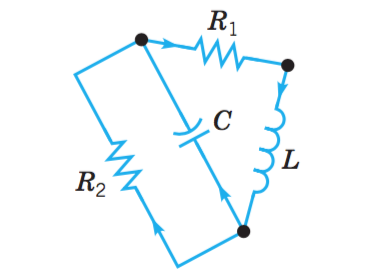
\includegraphics[width = 0.4\columnwidth]{finalReview2.png}
\end{figure}
How would you solve the system for this circuit? 
\par \textbf{Solution:} To derive the differential equation for a circuit, we need to use Kirchhoff's voltage law. This law states that the voltages drops around a closed loop will sum to zero. (This is essentially a statement of conservation of energy.) You can choose any loop (as long as your currents are consistent), but in this case well let $I_1$ be the current around the right loop, and $I_2$ be the current around the left loop. 
\par Left loop: 
\begin{gather*}
-R_2I_2 - \frac{(Q_2 - Q_1)}{C} = 0 \\
-R_2I_2 - \frac{\int I_2(\tau)d\tau - \int I_1(\tau)d\tau}{C} = 0\\
R_2I_2' + \frac{1}{C}I_2 - \frac{1}{C}I_1 = 0 \quad\blacksquare\\
\end{gather*}
\par Right loop: 
\begin{gather*}
-R_1I_1 - LI_1' - \frac{(Q_1 - Q_2)}{C} = 0\\
R_1I_1  + LI_1' + \frac{\int I_1(\tau)d\tau - \int I_2(\tau)d\tau}{C} = 0\\
LI_1'' +R_1I_1'  +  \frac{1}{C} I_1 - \frac{1}{C}I_2 = 0 \quad\blacksquare
\end{gather*}

\item \textbf{Power series:} Solve the following using a power series and give the recurrence relation. Write out your solution up to fifth order. Clearly state why you cannot use another method to solve the system.
\begin{enumerate}

% B&P 5.3 #16
\item $(2+x^2)y'' -xy' +4y=0, \quad y(0) = -1, \quad y'(0) = 3$
\par \textbf{Solution:} 
\begin{gather*}
(2+x^2)y'' -xy' +4y=0\\
2y'' + x^2y'' - xy' + 4y = 0\\
2\sum_{n=0}^\infty (n+2)(n+1)a_{n+2} x^n + x^2\sum_{n=0}^\infty (n+2)(n+1)a_{n+2} x^n  - x\sum_{n=0}^\infty (n+1) a_{n+1} x^n + 4\sum_{n=0}^\infty a_n x^n = 0\\
\sum_{n=0}^\infty (n+2)(n+1)a_{n+2} x^{n+2}  + \sum_{n=0}^\infty \left[ 2(n+2)(n+1)a_{n+2} + 4a_n\right]  x^n - \sum_{n=0}^\infty (n+1) a_{n+1} x^{n+1} = 0
\intertext{Reindexing the middle sum:}
m +2 = n\\
\sum_{n=0}^\infty (n+2)(n+1)a_{n+2} x^{n+2}  + \sum_{m=-2}^\infty \left[ 2(m+4)(m+3)a_{m+4} + 4a_{m+2}\right]  x^{m+2} - \sum_{n=0}^\infty (n+1) a_{n+1} x^{n+1} = 0
\intertext{Reindexing the right sum:}
m+2 = n+1\\
\sum_{n=0}^\infty (n+2)(n+1)a_{n+2} x^{n+2}  + \sum_{m=-2}^\infty \left[ 2(m+4)(m+3)a_{m+4} + 4a_{m+2}\right]  x^{m+2} - \sum_{m=-1}^\infty (m+2) a_{m+2} x^{m+2} = 0 \\
\sum_{n=0}^\infty (n+2)(n+1)a_{n+2} x^{n+2}  + \left[ 2(2)(1)a_{2} + 4a_{0}\right] + \left[ 2(3)(2)a_{3} + 4a_{1}\right]  x + \\
\qquad\qquad \qquad \sum_{m=0}^\infty \left[ 2(m+4)(m+3)a_{m+4} + 4a_{m+2}\right]  x^{m+2} - (1) a_{1} x - \sum_{m=0}^\infty (m+2) a_{m+2} x^{m+2} = 0 \\
\left[ 4a_{2} + 4a_{0}\right] + \left[ 12a_{3} + 3a_{1}\right]  x + \sum_{n=0}^\infty (n+2)(n+1)a_{n+2} x^{n+2}  + \\
\qquad\qquad\qquad\qquad \sum_{m=0}^\infty \left[ 2(m+4)(m+3)a_{m+4} + 4a_{m+2}\right]  x^{m+2} - \sum_{m=0}^\infty (m+2) a_{m+2} x^{m+2} = 0 \\
\left[ 4a_{2} + 4a_{0}\right] + \left[ 12a_{3} + 2a_{1}\right]  x +\\  
\sum_{n=0}^\infty\left[ (n+2)(n+1)a_{n+2}  + 2(n+4)(n+3)a_{n+4} + 4a_{n+2} - (n+2) a_{n+2} \right]x^{n+2} = 0 \\
\intertext{Matching coefficients to solve for the coefficients and recurrence relation:}
4a_2 + 4a_0 = 0 \implies a_2 = -a_0 \implies a_2 = 1\\
12a_3 + 3a_1 = 0 \implies a_3 = -\frac{1}{4}a_1\implies a_3 = -\frac{3}{4}\\
(n+2)(n+1)a_{n+2}  + 2(n+4)(n+3)a_{n+4} + 4a_{n+2} - (n+2) a_{n+2} = 0\\
n(n+2)a_{n+2}  + 2(n+4)(n+3)a_{n+4} + 4a_{n+2} = 0\\
a_{n+4} = \frac{-n(n+2)-4}{2(n+4)(n+3)}a_{n+2} \quad n \geq0
\intertext{Reindexing this:}
a_{n+2} =  \frac{-n(n-2)-4}{2(n+2)(n+1)}a_n \quad n \geq 2
\intertext{Solving for the higher coefficients:}
a_4 =  \frac{-4}{2(4)(3)}a_2  = -\frac{ 1}{6}\\
a_5 = \frac{-3(1)-4}{2(5)(4)}a_3 = \frac{21}{160}\\
\intertext{and writing out the solution up to fifth order:}
y(x) = -1 + 3x + x^2 - \frac{3}{4}x^3 - \frac{1}{6}x^4  + \frac{21}{160}x^5 + \cdots \quad\blacksquare
\end{gather*}

% B&P 5.3 17
\item $y'' + xy' + 2y = 0$
\par \textbf{Solution:} 
\begin{gather*}
y'' + xy' + 2y = 0 \\
\sum_{n=0}^\infty (n+2)(n+1)a_{n+2} x^n + x\sum_{n=0}^\infty (n+1) a_{n+1} x^n + 2\sum_{n=0}^\infty a_n x^n = 0 \\
\sum_{n=0}^\infty \left[(n+2)(n+1)a_{n+2} +2a_n\right]x^n + \sum_{n=0}^\infty (n+1) a_{n+1} x^{n+1} = 0 \\
\intertext{Reindex the first sum:}
m +1 = n\\
\sum_{m=-1}^\infty \left[(m+3)(m+2)a_{m+3} +2a_{m+1}\right]x^{m+1} + \sum_{n=0}^\infty (n+1) a_{n+1} x^{n+1} = 0 \\
\left[(2)(1)a_{2} +2a_{0}\right] + \sum_{m=0}^\infty \left[(m+3)(m+2)a_{m+3} +2a_{m+1}\right]x^{m+1} + \sum_{n=0}^\infty (n+1) a_{n+1} x^{n+1} = 0 \\
\left[2a_{2} +2a_{0}\right] + \sum_{n=0}^\infty \left[(n+3)(n+2)a_{n+3} +2a_{n+1}+ (n+1) a_{n+1} \right]x^{n+1} = 0 \\
\left[2a_{2} +2a_{0}\right] + \sum_{n=0}^\infty \left[(n+3)(n+2)a_{n+3} + (n+3) a_{n+1} \right]x^{n+1} = 0 \\
\intertext{Matching coefficients and finding the recurrence relation:}
2a_2 + 2a_0 = 0 \implies a_2 = -a_0\\
(n+3)(n+2)a_{n+3} + (n+3) a_{n+1}  = 0\implies a_{n+3} = \frac{-a_{n+1}}{n+2} \quad n \geq 0\\
\intertext{Reindexing the recurrence relation:}
a_{n+2} = \frac{-a_{n}}{n+1}\quad n \geq 1
\intertext{Solving for the higher coefficients:}
a_3 = -\frac{a_1}{2} \\
a_4 = \frac{-a_2}{3} = \frac{a_0}{3}\\
a_5 = \frac{-a_3}{4} = \frac{a_1}{4}\\
\intertext{and writing out the solution up to fifth order:}
y(x) = a_0 + a_1x - a_0x^2 - a_1x^3 + \frac{a_0}{2}x^4 + \frac{a_1}{3}x^5 + \cdots\\
y(x) = a_0\left(1  - x^2  + \frac{1}{3}x^4 + \cdots \right) + a_1\left(x - \frac{1}{2}x^3+\frac{1}{4}x^5 + \cdots\right) \quad\blacksquare
\end{gather*}

\end{enumerate}

\item \textbf{Direct method:} Consider the ODE
\[ y'' + x^2y = e^{-x}\]
Write out the direct method system of equations for the following boundary conditions for this ODE with $N=5$ nodes.
\begin{enumerate}

\item $y(0) = 0, \quad y(4) = 5$
\par \textbf{Solution:} 
\par We first need to write out the recursive equation:
\begin{gather*}
y'' + x^2y = e^{-x}\\
\frac{y_{i+1} - 2y_i + y_{i-1}}{h^2} + x_i^2y_i = e^{-x_i}\\
y_{i+1}+ (hx_i^2- 2)y_i + y_{i-1}= h^2e^{-x_i}
\end{gather*}
After this, we can apply the boundary conditions: 
\begin{gather*}
y_{3}+ (hx_2^2- 2)y_2 + y_{1}= h^2e^{-x_2} \\
y_{3}+ (hx_2^2- 2)y_2 + (0)= h^2e^{-x_2} \\
y_{3}+ (hx_2^2- 2)y_2= h^2e^{-x_2} \\
y_{5}+ (hx_4^2- 2)y_4 + y_{3}= h^2e^{-x_4} \\
5+ (hx_4^2- 2)y_4 + y_{3}= h^2e^{-x_4} \\
(hx_4^2- 2)y_4 + y_{3}= h^2e^{-x_4} - 5
\end{gather*}
Finally, we can set up the equations. (\textit{Note:} we will have three degrees of freedom.)
\[
\left[\begin{array}{ccc} 
(hx_2^2- 2) & 1 & 0\\
1 &  (hx_3^2- 2) & 1 \\
0 & 1 &  (hx_4^2- 2)\end{array} \right]
\left[ \begin{array}{c} y_2 \\ y_3 \\ y_4\end{array} \right] 
= \left[ \begin{array}{c} h^2e^{-x_2} \\ h^2e^{-x_3} \\ h^2e^{-x_4} - 5\end{array} \right] \quad\blacksquare
\]

\item $y(0) = 0, \quad 4y'(2) +  3y(2)= 5$
\par \textbf{Solution:}
\par We only need to change the boundary conditions since this is the same ODE and thus has the same recursive equation:
\begin{gather*}
y_{3}+ (hx_2^2- 2)y_2 + y_{1}= h^2e^{-x_2} \\
y_{3}+ (hx_2^2- 2)y_2 + (0)= h^2e^{-x_2} \\
y_{3}+ (hx_2^2- 2)y_2= h^2e^{-x_2} \\
y_{6}+ (hx_5^2- 2)y_5 + y_{4}= h^2e^{-x_5} \\
4\frac{y_6 - y_4}{2h} + 3y_5 = 5\\
y_6 = \frac{5}{2}h-\frac{3}{2}hy_5 +y_4\\
 \frac{5}{2}h-\frac{3}{2}hy_5 +y_4 + (hx_5^2- 2)y_5 + y_{4}= h^2e^{-x_5}\\
 \left(hx_5^2- 2-\frac{3}{2}h\right)y_5 + 2y_4 = h^2e^{-x_5} - \frac{5}{2}h
\end{gather*}

Finally, we set up the equations. (\textit{Note:} here we will have four degrees of freedom because of the right boundary condition.)
\[
\left[\begin{array}{cccc} 
(hx_2^2- 2) & 1 & 0&0\\
1 &  (hx_3^2- 2) & 1&0 \\
0 & 1 &  (hx_4^2- 2)&1\\
0&0 & 2& hx_5^2- 2-\frac{3}{2}h\end{array} \right]
\left[ \begin{array}{c} y_2 \\ y_3 \\ y_4\\y_5 \end{array} \right] 
= \left[ \begin{array}{c} h^2e^{-x_2} \\ h^2e^{-x_3} \\ h^2e^{-x_4} \\h^2e^{-x_5} - \frac{5}{2}h\end{array} \right] \quad\blacksquare
\]

\end{enumerate}

\item \textbf{Numerical methods:} Write a short piece of MATLAB code to solve the following using backward Euler.
\[ y' + 5y^2 = \sin(x), \quad y(0) = 10\]
\par \textbf{Solution:} To use backward Euler, we need to write out the definition of backward Euler then resolve for $y_{i+1}$:

\begin{align*}
y_{i+1} &= y_i + hy'(x_{i+1},y_{i+1})\\
y' &= \sin(x) - 5y^2\\
y_{i+1} &= y_i + h\left[ \sin(x_{i+1}) - 5y_{i+1}^2\right] \\
y_{i+1} &= y_i + h \sin(x_{i+1}) - 5hy_{i+1}^2 \\
\end{align*}
Note that this is a quadratic equation for $y_{i+1}$, so we can solve this to find a closed-form solution for $y_{i+1}$:
\begin{gather*}
y_{i+1} = y_i + h \sin(x_{i+1}) - 5hy_{i+1}^2 \\
5hy_{i+1}^2 + y_{i+1} - (y_i + h \sin(x_{i+1})) = 0\\
y_{i+1} = \frac{-1 \pm\sqrt{1 - 4(5h)(y_i+h\sin(x_{i+1}))}}{10h}
\end{gather*}

From here we can write out the MATLAB function to solve this ODE:

\begin{lstlisting} 
y(1) = 10; 
x(1) = 0;
i = 1;
while x < xmax
	x(i+1) = x(i) + h;
	y(i+1) = (-1 + sqrt(1 - 4*5*h*(y(i) + h*sin(x(i+1)))))/10/h;
	i = i+1;
end

\end{lstlisting}

\end{enumerate}

%----------------------------------------------------------------------------------------

\end{document}